\begin{figure}[h]
\begin{minipage}{0.3\columnwidth}
\resizebox{\columnwidth}{!}{
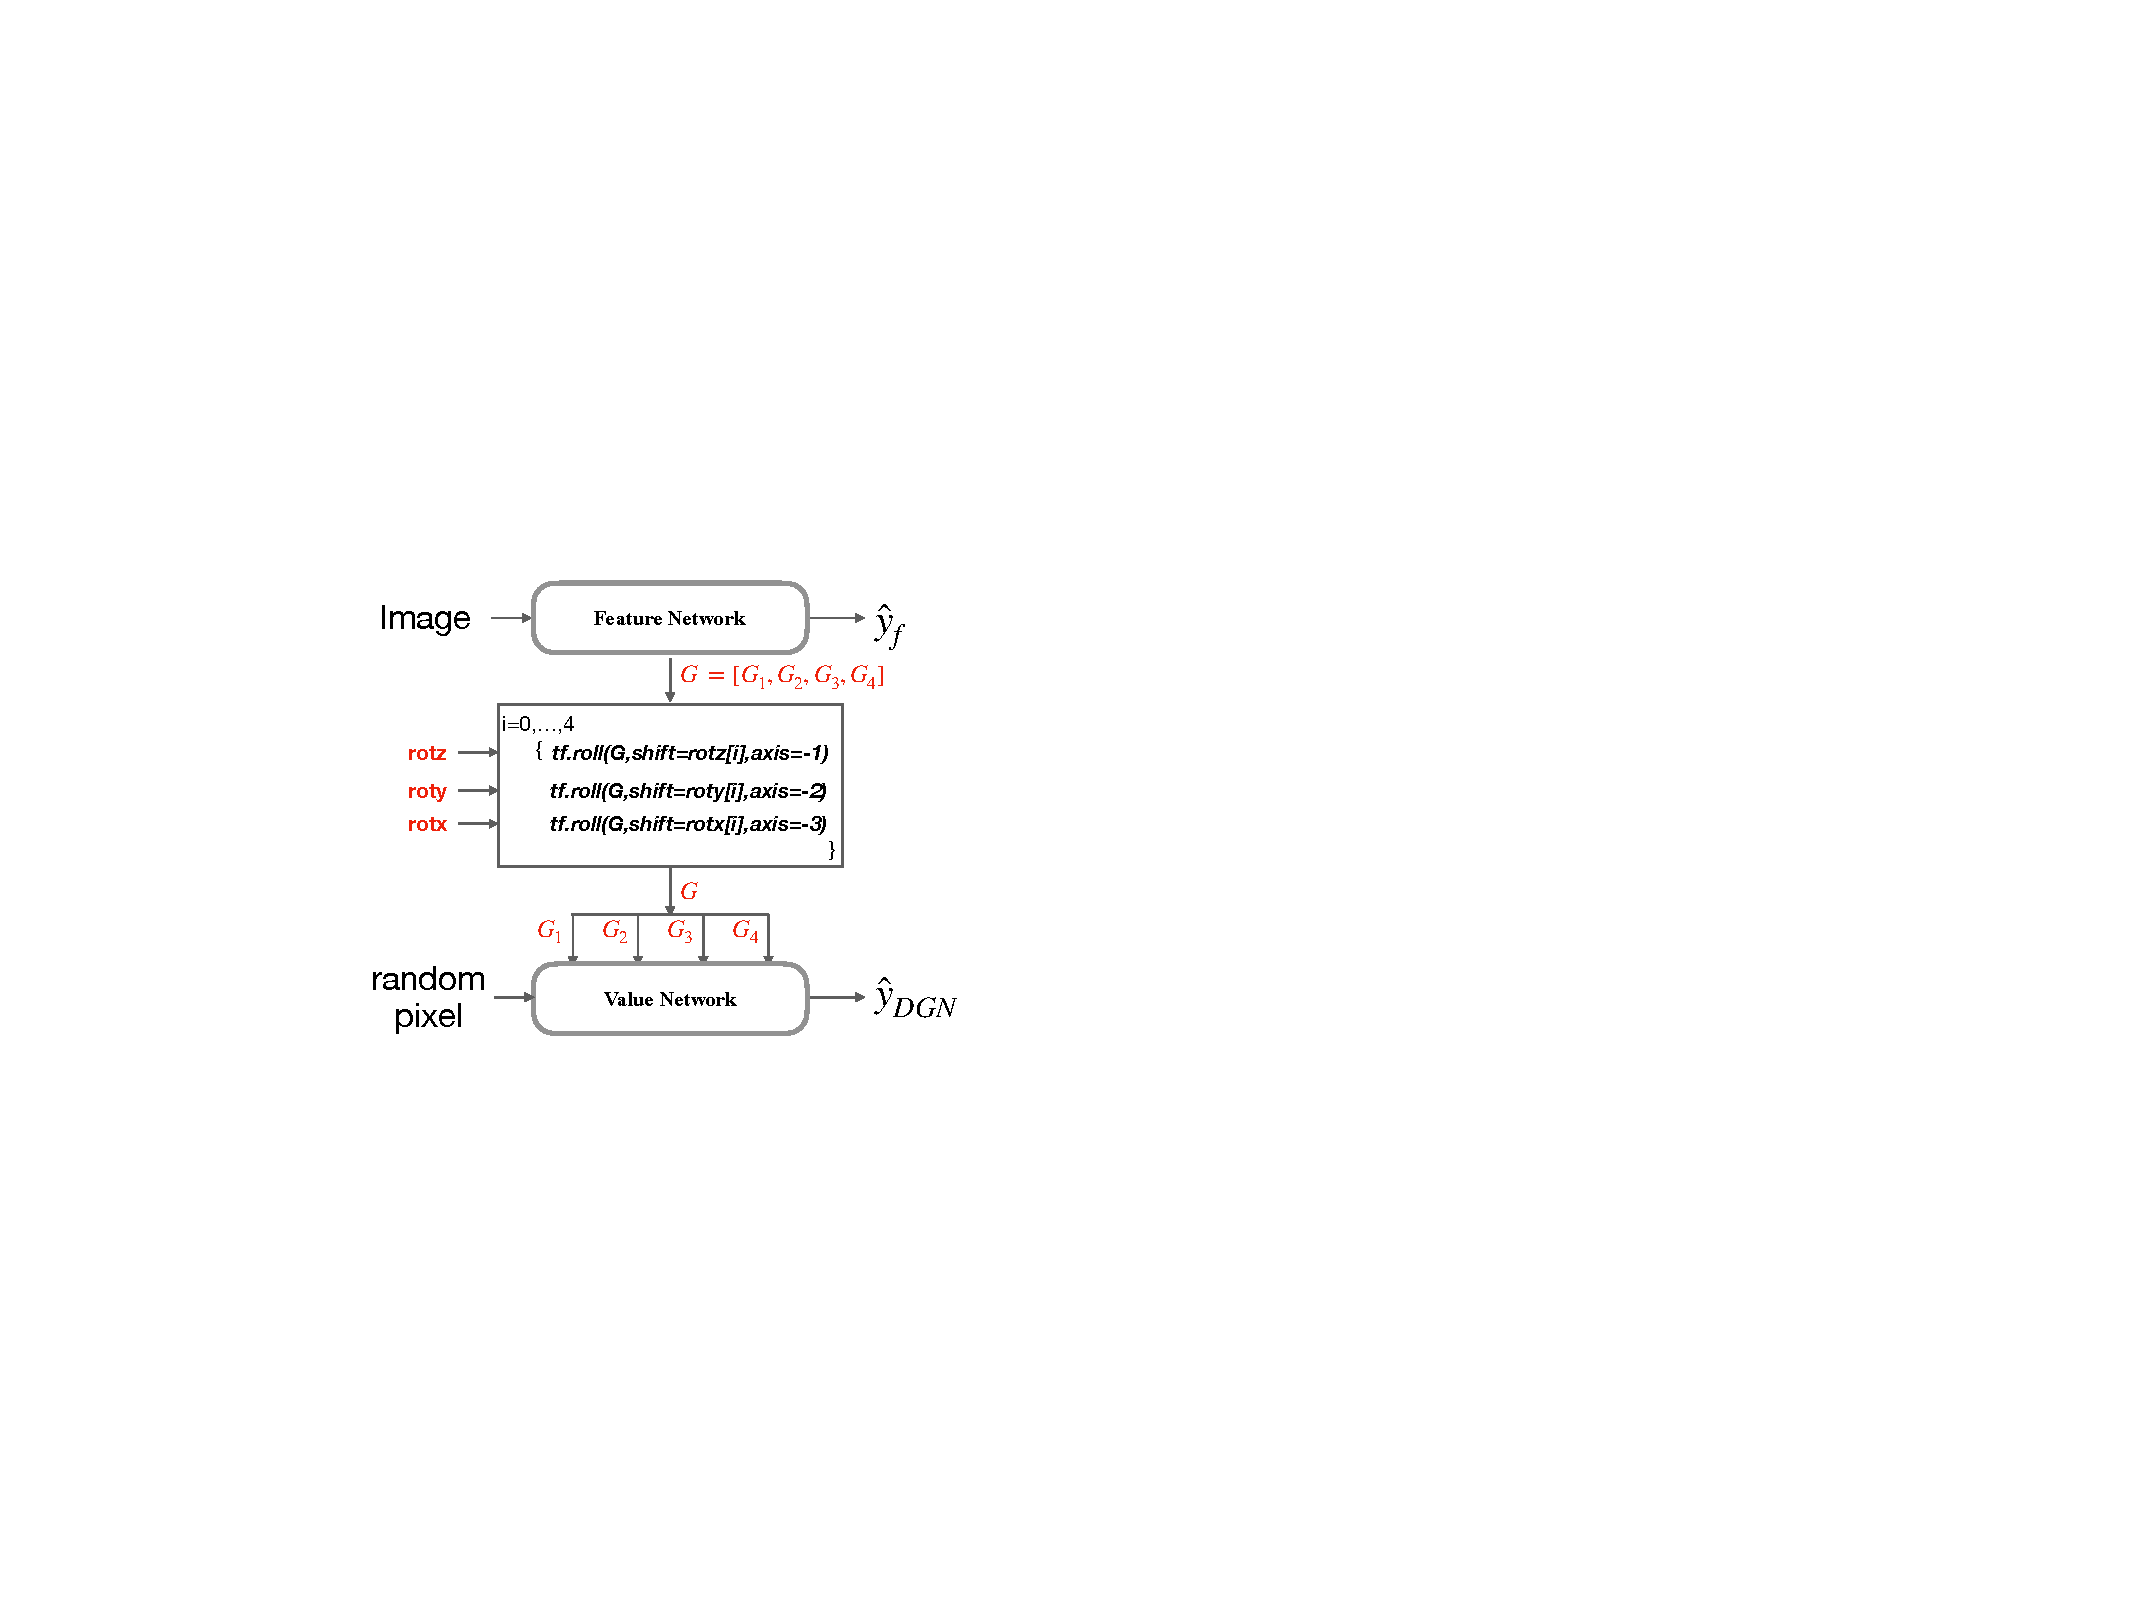
\includegraphics[scale=0.25]{figs/arbitrary_shift.pdf}
}
\end{minipage}
\begin{minipage}{0.68\columnwidth}
\resizebox{\columnwidth}{!}{
\includegraphics{visual-iclr/images/horse.png}
\includegraphics{visual-iclr/images/original/layer_1_0.png}
\includegraphics{visual-iclr/images/original/layer_1_1.png}
\includegraphics{visual-iclr/images/original/layer_2_0.png}
\includegraphics{visual-iclr/images/original/layer_2_1.png}
\includegraphics{visual-iclr/images/original/layer_3_0.png}
\includegraphics{visual-iclr/images/original/layer_3_1.png}
\includegraphics{visual-iclr/images/original/layer_4_0.png}
\includegraphics{visual-iclr/images/original/layer_4_1.png}
}\\
\resizebox{\columnwidth}{!}{
\includegraphics{visual-iclr/images/randinput.png}
\includegraphics{visual-iclr/images/permuted/layer_1_0.png}
\includegraphics{visual-iclr/images/permuted/layer_1_1.png}
\includegraphics{visual-iclr/images/permuted/layer_2_0.png}
\includegraphics{visual-iclr/images/permuted/layer_2_1.png}
\includegraphics{visual-iclr/images/permuted/layer_3_0.png}
\includegraphics{visual-iclr/images/permuted/layer_3_1.png}
\includegraphics{visual-iclr/images/permuted/layer_4_0.png}
\includegraphics{visual-iclr/images/permuted/layer_4_1.png}
}
\end{minipage}
\caption{Top (Standard CNN): First image on the left is the input image and the next $8$ images are outputs of $2$ filters in each of the $4$ layers. Bottom (DGN with gates of the top model applied in reverse order): First image on the left is the input to the value network and the next $8$ images are outputs of $2$ filters in each of the $4$ layers. Both models achieve a test accuracy of about $80\%$.}
\label{fig:visual-permute}
\end{figure}
